\documentclass{book}
%\documentclass{article}           %for shorter notes
\usepackage{graphicx}              %for PNG images (pdflatex)
%\usepackage{graphics}              %for EPS images (latex)
\usepackage[linkbordercolor={1.0 1.0 0.0}]{hyperref}  %for \url tag
\usepackage{color}                 %for defining custom colors
\usepackage{framed}                %for shaded and framed paragraphs
\usepackage{textcomp}              %for various symbols, e.g. Registered Mark
\usepackage{geometry}              %for defining page size
\usepackage{longtable}             %for breaking tables
\usepackage{multirow}
\usepackage{booktabs}
\usepackage{ltablex}
\usepackage[table]{xcolor} % Note: The rowcolors command does not work properly with the tabularx environment.

%
\geometry{verbose,a4paper,tmargin=2.5cm,bmargin=2.5cm,lmargin=2.5cm,rmargin=2cm}
\hypersetup{
  pdfauthor = {KnowARC collaboration},
  pdftitle = {libarcclient},
  pdfsubject = {A Client Library for ARC},
  pdfkeywords = {ARC,client,library},
  pdfcreator = {PDFLaTeX with hyperref package},
  pdfproducer = {PDFLaTeX}
}
%
\bibliographystyle{IEEEtran}       %a nice bibliography style
%
\def\efill{\hfill\nopagebreak}%
\hyphenation{Nordu-Grid}
\setlength{\parindent}{0cm}
\setlength{\FrameRule}{1pt}
\setlength{\FrameSep}{8pt}
\addtolength{\parskip}{5pt}
\renewcommand{\thefootnote}{\fnsymbol{footnote}}
\renewcommand{\arraystretch}{1.3}
\newcommand{\dothis}{\colorbox{shadecolor}}
\newcommand{\globus}{Globus Toolkit\textsuperscript{\textregistered}~2~}
\newcommand{\GT}{Globus Toolkit\textsuperscript{\textregistered}}
\newcommand{\ngdl}{\url{http://ftp.nordugrid.org/download}~}
\newcommand{\libarcclient}{libarcclient}
\newcommand{\ACC}{\texttt{ACC}}
\newcommand{\ACCConfig}{\texttt{ACCConfig}}
\newcommand{\Config}{\texttt{Config}}
\newcommand{\Broker}{\texttt{Broker}}
\newcommand{\Random}{\texttt{Random}}
\newcommand{\Benchmark}{\texttt{Benchmark}}
\newcommand{\FastestQueueBroker}{\texttt{FastestQueueBroker}}
\newcommand{\PythonBroker}{\texttt{PythonBroker}}
\newcommand{\Data}{\texttt{Data}}
\newcommand{\ClientInterface}{\texttt{ClientInterface}}
\newcommand{\ClientTCP}{\texttt{ClientTCP}}
\newcommand{\ClientHTTP}{\texttt{ClientHTTP}}
\newcommand{\ClientSOAP}{\texttt{ClientSOAP}}
\newcommand{\ExecutionTarget}{\texttt{ExecutionTarget}}
\newcommand{\Job}{\texttt{Job}}
\newcommand{\JobController}{\texttt{JobController}}
\newcommand{\JobDescription}{\texttt{JobDescription}}
\newcommand{\JobSupervisor}{\texttt{JobSupervisor}}
\newcommand{\Loader}{\texttt{Loader}}
\newcommand{\Logger}{\texttt{Logger}}
\newcommand{\TargetGenerator}{\texttt{TargetGenerator}}
\newcommand{\TargetRetriever}{\texttt{TargetRetriever}}
\newcommand{\Sandbox}{\texttt{Sandbox}}
\newcommand{\Submitter}{\texttt{Submitter}}
\newcommand{\URL}{\texttt{URL}}
\newcommand{\UserConfig}{\texttt{UserConfig}}
\newcommand{\XML}{\texttt{XML}}
\newcommand{\XMLNode}{\texttt{XMLNode}}
\newcommand{\NST}[1]{\normalsize{\textnormal{#1}}}
\newcommand{\defineheadfoot}{\endfirsthead %
\midrule %
\multicolumn{5}{c}{Continued from previous page}\\%
\midrule %
\endhead %
\midrule %
\multicolumn{5}{c}{Continues at next page}\\%
\midrule %
\endfoot %
\bottomrule %
\endlastfoot}
\definecolor{shadecolor}{rgb}{1,1,0.6}
\definecolor{salmon}{rgb}{1,0.9,1}
\definecolor{bordeaux}{rgb}{0.75,0.,0.}
\definecolor{cyan}{rgb}{0,1,1}

\colorlet{tableheadcolor}{gray!25}
\colorlet{tablerowcolor}{gray!12.5}

\newcolumntype{C}{>{\ttfamily\footnotesize}c}
\newcolumntype{T}{>{\ttfamily\footnotesize\centering\arraybackslash}X}

%
%----- DON'T CHANGE HEADER MATTER
\begin{document}
\def\today{\number\day/\number\month/\number\year}

\begin{titlepage}

\begin{tabular}{rl}
\resizebox*{3cm}{!}{
\includegraphics{ng-logo.png}}
&\parbox[b]{2cm}{\textbf \it {\hspace*{-1.5cm}NORDUGRID\vspace*{0.5cm}}}
\end{tabular}

\hrulefill

%-------- Change this to NORDUGRID-XXXXXXX-NN

{\raggedleft NORDUGRID-TECH-20\par}

{\raggedleft \today\par}

\vspace*{2cm}

%%%%---- The title ----
{\centering \textsc{\Large {\libarcclient}}\Large \par}
\vspace*{0.5cm}

%%%%---- A subtitle, if necessary ----
{\centering \textit{\large A Client Library for ARC}\large \par}

\vspace*{1.5cm}
%%%%---- A list of authors ----
{\centering \large KnowARC \large \par}
%%%%---- An abstract - if style is article ----
%\begin{abstract}
%The abstract
%\end{abstract}
\end{titlepage}

\tableofcontents                   %Comment if use article style
\newpage
\chapter{Preface}
\label{sec:intro}

This document describes from a technical viewpoint a plugin-based
client library for the new Web Service (WS) based Advanced Resource
Connector~\cite{arc} (ARC) middleware. The library consists of a set
of C++ classes for

\begin{itemize}
\item{handling proxy, user and host certificates,}
\item{performing computing resource discovery and information retrieval,}
\item{filtering and brokering of found computing resources,}
\item{job submission and management and}
\item{data handling.}
\end{itemize}

All capabilities are enabled for three different grid flavours
(Production ARC, Web Service ARC and gLite~\cite{glite}) through a
modular design using plugins specialized for each supported
middleware. Future extensions to support additional middlewares
involve plugin compilation only i.e., no recompilation of main
libraries or clients is necessary.

Using the library, a set of command line tools have been built which
puts the library's functionality at the fingertips of users. This
documentation is not intended to document the developed CLI but the
concept of how to build command line tools will be
demonstrated. Readers interested in the user interface are recommended
to read the client user manual~\cite{ui}.

\chapter{Functionality Overview}
\label{sec:FuncOver}

The new {\libarcclient} makes extensive use of plugins for command
handling. These plugins are handled by a set of higher level classes
which thus are the ones to offer the plugin functionality to external
calls. In this section an overview of the library's main functionality
is given which also introduces the most important higher level
classes. Readers interested in the library API are recommended to look
up the online API documentation~\cite{libarcclientAPI}.

\section{Resource Discovery and Information Retrieval}
\label{sec:TargetDiscovery}

With the increasing number of grid clusters around the world, a
reliable and fast resource discovery and information retrieval
capability is of crucial importance for a user interface. The new
{\libarcclient} resource discovery and information retrieval component
consists of three classes; the {\TargetGenerator}, the
{\TargetRetriever} and the {\ExecutionTarget}. Of these the
{\TargetRetriever} is a base class for further grid middleware
specific specialization (plugin).

Figure \ref{fig:ResDisc} depicts how the classes work together in a
command chain to discover all resources registered with a certain
information server. Below a description of each step is given:

\begin{figure}[ht]
\centering{{\scalebox{0.75}{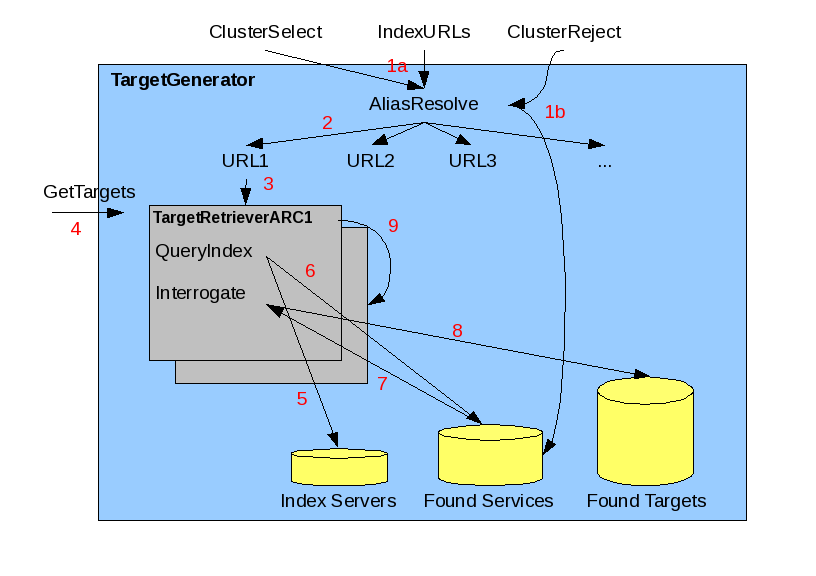
\includegraphics{TargetDiscovery.png}}}
\caption{\label{fig:ResDisc}Diagram depicting the resource discovery
  and information retrieval process}}
\end{figure}

\begin{enumerate}
\item{The {\TargetGenerator} takes three arguments as input. The first
  argument is a reference to a {\UserConfig} object containing a
  representation of the contents of the user's configuration file. The
  second and third arguments contain lists of strings. The first list
  contains individually selected and rejected computing services,
  while the second list contains individually selected and rejected
  index servers. Rejected servers and services are identified by that
  its name is prefixed by a minus sign in the lists. The name of the
  servers and services should be given either in the form of an alias
  defined in the {\UserConfig} object or as the name of its grid
  flavour followed by a colon and the URL of its information contact
  endpoint.}
\item{These lists are parsed through alias resolution before being
  used to initialize the complete list of selected and rejected
  {\URL}s pointing to computing services and index servers.}
\item{For each selected index server and computing service a
  {\TargetRetriever} plugin for the server's or service's grid flavour
  is loaded using the ARC loader. The {\TargetRetriever} is
  initialized with its {\URL} and the information about whether it
  represents a computing service or an index server.}
\item{An external call is received calling for targets to be
  prepared. The call for targets is processed by each
  {\TargetRetriever} in parallel.}
\item{A {\TargetRetriever} representing an index server first tries to
  register at the index server store kept by the {\TargetGenerator}.
  If allowed to register, the index server is queried and the query
  result processed. The {\TargetGenerator} will not allow
  registrations from index servers present in its list of rejected
  index servers or from servers that have already registered
  once. Index servers often register at more than one index server,
  thus different {\TargetRetriever}s may discover the same server.}
\item{If while processing the query result the {\TargetRetriever}
  finds another registered index server or a registered computing
  service it creates a new {\TargetRetriever} for the found server or
  service and forwards the call for targets to the new
  {\TargetRetriever}.}
\item{A {\TargetGenerator} representing a computing service first
  tries to register at the service store kept by the
  {\TargetGenerator}. If allowed to register, the computing server is
  queried and the query result processed. The {\TargetGenerator} will
  not allow registrations from computing services present in its list
  of rejected computing services or from service that have already
  registered once. Computing services often register at more than one
  index server, thus different {\TargetRetriever}s may discover the
  same service.}
\item{When processing the query result the {\TargetRetriever} will
  create an {\ExecutionTarget} for each queue found on the computing
  service and collect all possible information about them. It will
  then store the {\ExecutionTarget} in the found targets store kept
  by the {\TargetGenerator} for later usage (e.g.\ status printing or
  job submission).}
\end{enumerate}

\section{Job Submission}
\label{sec:JobSubmission}

Job submission starts with the resource discovery and target
preparation as outlined in the Section~\ref{sec:TargetDiscovery}. Not
until a list of possible targets (which authorize the user) is available
is the job description read in order to enable bulk job submission of
widely different jobs without having to reperform the resource
discovery. In addition to the classes mentioned above the job
submission makes use of the {\Broker}, {\JobDescription} and
{\Submitter} classes.  The {\Submitter} is base class for further grid
middleware specific specialization (plugin) similarly to the {\TargetRetriever}.

\begin{figure}[ht]
\centering{{\scalebox{0.75}{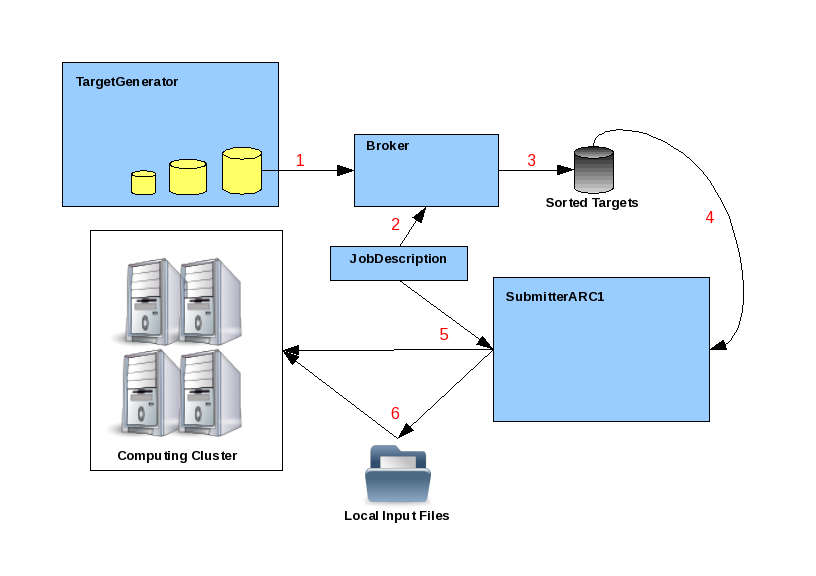
\includegraphics{JobSubmission.png}}}
\caption{\label{fig:JobSub}Diagram depicting the submission of a job
  to a computing service.}}
\end{figure}

Figure \ref{fig:JobSub} shows a job submission sequence and below a
description of each step is given:

\begin{enumerate}
\item{The {\TargetGenerator} has prepared a list of
  {\ExecutionTarget}s. Depending on the {\URL}s provided to the
  {\TargetGenerator} the list of found {\ExecutionTarget}s may be
  empty or contain several targets. Targets may even represent more
  than one grid flavour. The list of found targets are given as input
  to the {\Broker}.}
\item{In order to rank the found services ({\ExecutionTarget}s) the
  {\Broker} needs detailed knowledge about the job requirements, thus
  the {\JobDescription} is passed as input to the brokering process.}
\item{The {\Broker} filters and ranks the {\ExecutionTarget}s according
  to the ranking method chosen by the user.}
\item{Each {\ExecutionTarget} has a method to return a specialized
  {\Submitter} which is capable of submitting jobs to the service it
  represents. The best suitable {\ExecutionTarget} for the job is
  asked to return a {\Submitter} for job submission.}
\item{The {\Submitter} takes the {\JobDescription} as input and
  uploads it to the computing service.}
\item{The {\Submitter} identifies local input files from the
  {\JobDescription} and uploads them to the computing service.}
\end{enumerate}

\section{Job Management}
Once a job is submitted, job related information (job identification
string, cluster etc.) is stored in a local XML file which stores this
information for all active jobs. This file may contain jobs running on
completely different grid flavours, and thus job management should be
handled using plugins similar to resource discovery and job
submission. The job managing plugin is called the {\JobController} and
it is supported by the {\JobSupervisor} and {\Job} classes.

\begin{figure}[ht]
\centering{{\scalebox{0.75}{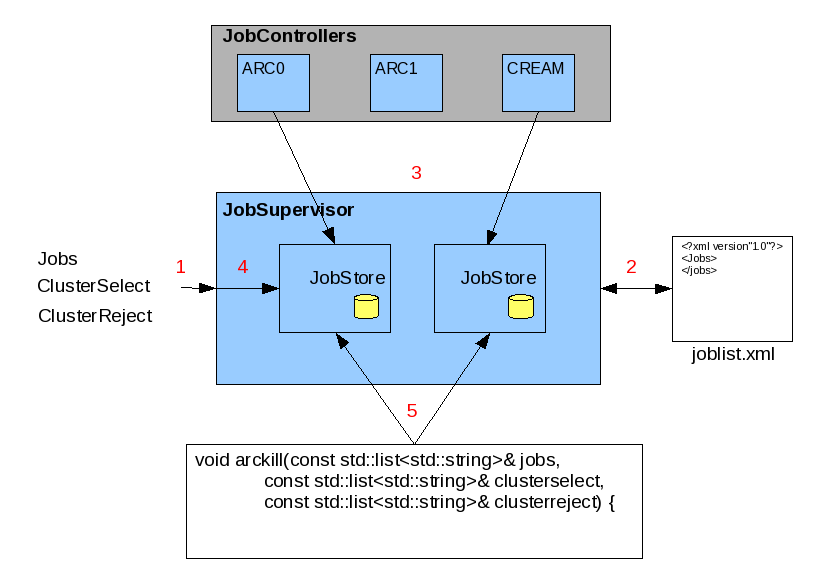
\includegraphics{JobManagement.png}}}
\caption{\label{fig:JobMan}Diagram depicting how job controlling
  plugins, {\JobController}s, are loaded and initialized.}}
\end{figure}

Figure~\ref{fig:JobMan} shows how the three different classes work
together and below a step by step description is given:

\begin{enumerate}
\item{The {\JobSupervisor} takes four arguments as input. The first
  argument is a reference to a {\UserConfig} object containing a
  representation of the contents of the user's configuration file. The
  second is a list of strings containing job identifiers and job
  names, the third is a list of strings of clusters to select or
  reject (in the same format as described for the {\TargetGenerator}
  above). The last argument is the name of the file containing the
  local information about active jobs, hereafter called the joblist
  file.}
\item{A job identifier does not uniquely define which grid flavour
  runs a certain job. Thus this information is stored in the joblist
  file upon submission by the {\Submitter} and the joblist file is
  extensively used by the {\JobSupervisor} to identify the
  {\JobController} flavours which are to be loaded. The information in
  the joblist file is also used to look up the job identifier for jobs
  specified using job names. Alias resolving for the selected and
  rejected clusters are performed using the information in the
  {\UserConfig} object.}
\item{Suitable {\JobController}s are loaded}
\item{The list of job identifiers and selected and rejected clusters
  are passed to each {\JobController} which uses the information to
  fill its internal \texttt{JobStore}.}
\item{Residing within the {\JobSupervisor} the {\JobController}s are
  now accessible for external calls (i.e. job handling).}
\end{enumerate}

\chapter{The ARC Brokering Module}
\label{sec:brokering}
The ARC brokering module is made up of two kinds of classes: one
brokering base class and specialized classes derived thereof. The
brokering base class which implements the method for reducing a list
of resources found by resource discovery (the list of
{\ExecutionTarget}s residing within the {\TargetGenerator}) to a list
of resources capable of running a certain job:

\begin{shaded}
\begin{verbatim}
void PreFilterTargets(const TargetGenerator& targen, const JobDescription& jd);
\end{verbatim}
\end{shaded}

The {\texttt PreFilterTargets} method compares every hardware and
software requirement given in the job description against the
computing resource (cluster) specifications stored in the
{\ExecutionTarget}. If the{\ExecutionTarget} doesn't fulfil the
requirements imposed by the job description, or it is impossible to
carry out the matchmaking due to incomplete information published by
the computing resource, the {\ExecutionTarget} will be removed from
the list of possible targets. A detailed overview of the matchmaking
between {\JobDescription} and {\ExecutionTarget} attributes is given
in Appendix~\ref{app:broker-mapping}.

Once prefiltered, the remaining {\ExecutionTarget}s should be ranked
in order to return the ``best'' {\ExecutionTarget} for job
submission. Different ranking methods are implemented by the
specialized brokers, but for usability and consistency reasons these
methods are encapsulated by the {\Broker} base class method

\begin{shaded}
\begin{verbatim}
ExecutionTarget& GetBestTarget(bool &EndOfList);
\end{verbatim}
\end{shaded}

which invokes the {\texttt SortTargets} method implemented by the
specialized broker (see Section~\ref{sec:brokerplugins}) and returns
the best target. The {\texttt GetBestTarget} method is ``incremented''
at each call, thus upon a second call the second best
{\ExecutionTarget} will be returned.

\section{Broker plugins}
\label{sec:brokerplugins}

\subsubsection{\Random}

The {\Random} ranks the {\ExecutionTarget}s randomly.

\subsection{\Benchmark}

The {\Benchmark} ranks the {\ExecutionTarget}s according to their
benchmark performance. Through the command line tool (see the user
manual\cite{ui} for reference) this specialized broker takes a user
specified benchmark as input and ranks the {\ExecutionTarget}s
according to their published benchmark performance. If no benchmark is
specified the CINT2000 (Integer Component of SPEC
CPU2000)\footnote{http://www.spec.org/cpu2000/CINT2000/} benchmark is
used as default.

\subsection{\FastestQueueBroker}

The {\FastestQueueBroker} ranks the {\ExecutionTarget}s according to
their queue length measured in percentage of the {\ExecutionTarget}'s
size (i.e. the queue length divided by the number of total
slots/CPUs). If more than one {\ExecutionTarget} has zero queue, the
{\FastestQueueBroker} makes use of a basic load balancing method to
rearrange the zero queue {\ExecutionTarget}s depending on their number
of free slots/CPUs.

\subsection{\Data}

The {\Data} ranks the {\ExecutionTarget}s according to how many
megabytes of the requested input files that already stored in the
cache of the computing resource the {\ExecutionTarget} represents. The
broker is motivated by that jobs should be submitted to
{\ExecutionTarget}s where the data already is, thus reducing the
network load on both the computing resource and client side. The
ranking method is based upon the
A-REX\footnote{http://www.knowarc.eu/download/D1.2-3\_documentation.pdf}
interface {\texttt CacheCheck} for querying for the presence of the
file in the cache directory. This interface has a limitation in the
current implementation and does not support per user caches.

The {\texttt SortTargets} method has four steps:

\begin{enumerate}
\item{Only the A-REX service has {\texttt CacheCheck} method, thus
  {\ExecutionTarget}s not running A-REX are removed.}
\item{Information about input files requested in the job description
  is collected from the \texttt{JobInnerRepresentation.}}
\item{Each {\ExecutionTarget} is queried (through the {\texttt
    CacheCheck} method) for the existence of input files.  A single
  query is used for achieving all the necessary information and file
  sizes are summarized. If there are problems determining file sizes,
  then the summarized size will be zero.}
\item{The possible {\ExecutionTarget}s are ranked in a descending
  order according to the amount of input data they have in their
  cache.}
\end{enumerate}

Example of a CacheCheck request that can be sent to an A-REX service:

\begin{shaded}
\begin{verbatim}
<CacheCheck>
   <TheseFilesNeedToCheck>
       <FileURL>http://knowarc1.grid.niif.hu/storage/Makefile</FileURL>
       <FileURL>ftp://download.nordugrid.org/test/README</FileURL>
   </TheseFilesNeedToCheck>
</CacheCheck>
\end{verbatim}
\end{shaded}

Example CacheCheck response from the A-REX service:

\begin{shaded}
\begin{verbatim}
<CacheCheckResponse>
   <CacheCheckResult>
   <Result>
         <FileURL>http://knowarc1.grid.niif.hu/storage/Makefile</FileURL>
         <ExistInTheCache>true</ExistInTheCache>
         <FileSize>190</FileSize>
   </Result>
   <Result>
         <FileURL>ftp://download.nordugrid.org/test/README</FileURL>
         <ExistInTheCache>true</ExistInTheCache>
         <FileSize>176</FileSize>
   </Result>
  </CacheCheckResult>
</CacheCheckResponse>
\end{verbatim}
\end{shaded}

\subsection{\PythonBroker}

This {\PythonBroker} allows users to write their customized broker in
python. To use this broker the user should write a python class which
should contain:

\begin{itemize}

\item{an \_\_init\_\_ method that takes a Config object as input, and}
\item{a SortTargets method that takes a python list of ExecutionTarget
  objects and a JobInnerRepresentation object as input.}

\end{itemize}

The {\Config}, {\ExecutionTarget} and {\texttt JobInnerRepresentation} classes are
available in the swig generated arc python module.

To invoke the {\PythonBroker}, the name of the python module defining
the broker class and the name of the broker class must be given. If
e.g. the broker class MyBroker is defined in the python module
SampleBroker the command line option to arcsub to use this broker is:

\begin{shaded}
\begin{verbatim}
-b PythonBroker:SampleBroker.MyBroker
\end{verbatim}
\end{shaded}

Additional arguments to the python broker can be added by appending
them after an additional colon after the python class name:

\begin{shaded}
\begin{verbatim}
-b PythonBroker:SampleBroker.MyBroker:args
\end{verbatim}
\end{shaded}

Extracting these additional arguments should be done in the python
broker class's \_\_init\_\_ method.

For a complete example of a simple python broker see the
SampleBroker.py file that comes with your arc python installation.

\chapter{Job Description}
\label{sec:jobdesc}

\chapter{Grid Flavour Plugins)}
\label{sec:plugins}

\section{ARC0 Plugins}

The ARC0 plugins enables support for the interfaces used by computing
elements running ARC version 0.x.

The ARC 0.x local information system uses the {\GT}~\cite{globus} GRIS
with a custom made ARC schema. The information index server used is the
{\GT} GIIS. Both these servers use the LDAP~\cite{ldap}
protocol. The specialization of the {\TargetRetriever} class for ARC0
is implemented using the ARC LDAP Data Management Component (DMC) (see
\cite{hed} for technical details).

Jobs running on an ARC 0.x computing element are handled by the ARC
grid-manager~\cite{gm}. Job submission and job control are done using
the gridftp~\cite{gridftp} protocol. The specializations of the
{\Submitter} and {\JobController} classes use the globus ftp control
library.

Stage-in and stage-out of input and output files are also done using
the gridftp~\cite{gridftp} protocol. This means that proper
functionality of the ARC0 plugins requires the gridftp DMC.

\section{ARC1 Plugins}

The computing element in ARC version 1.x is the A-Rex~\cite{arex}
service running in a HED~\cite{hed} container.

A-Rex implements the BES~\cite{ogsa-bes} standard interface. Since
this is a SOAP-based~\cite{soap} interface, the specializations of the
{\TargetRetriever}, {\Submitter} and {\JobController} classes make use
of a chain of ARC Message Chain Components (MCC~\cite{hed}) ending
with the SOAP client MCC.

The A-Rex service uses the https protocol \texttt{put} and \texttt{get} methods for
stage-in and stage-out of input and output files. Therefore, the ARC1
plugins requires the http DMC.

\section{gLite Plugins}

The gLite computing element offers several interfaces, one of them
being the Web Service based computing element interface known as the
CREAM CE~\cite{cream}. The current revision of this interface (CREAM
version 2) has been chosen for implementation within {\libarcclient} for the
following reasons:

\begin{itemize}
\item CREAM2 has a Web Service interface that is very similar to the Web Service
  based ARC.
\item CREAM2 enables direct access to the gLite computing element
  without having to go via the gLite workload management system.
\item CREAM2 contains numerous improvements when compared to the
  earlier CREAM versions.
\item CREAM2 supports direct job status queries.
\item CREAM2 offers a convenient way of handling input and output
  files through accessing the input and output sandbox via GridFTP.
\end{itemize}

gLite resources are registered in top level and site BDIIs. The CREAM
specialization of the {\TargetRetriever} therefore makes use of the
LDAP DMC similarly to the ARC0 plugins.

CREAM has its own SOAP-based interface. The CREAM
specializations of the {\Submitter} and {\JobController} classes
therefore use an MCC chain ending with the SOAP client MCC the same
way the ARC1 plugin does.

Stage-in and stage-out of input and output files are done using the
gridftp protocol. The gridftp DMC is therefore required.

\appendix

\chapter{{\ExecutionTarget}}
\label{app:ExTarget}

http://svn.nordugrid.org/trac/nordugrid/browser/arc1/trunk/doc/client/ExecutionTargetMapping.html

\chapter{Broker mapping}
\label{app:broker-mapping}

This document contains a description of the broker used in the Advanced
Resource Connector (ARC) middleware as of version 1.0. In section
\ref{sec:Attribute-matching} a description of how target attributes
are matched and compared to attributes specified in the job description.

In the broker attributes published by the candidate target need to
be matched and compared to attributes specified in the job description
to be able to select targets which are suitable for accepting the
job description. Targets which do not pass a certain comparison will
be not be a candidate target for submission. Detailed information
about the attributes described below can be found in the ARC job description
document. First the broker will check some basics for the target being
processed. First, if the job description specifies submission to specific
targets and/or queues, the target will be checked and if it is not
among these targets and/or queues, it will be dropped. Next the number
of free slots on the target will be checked, and if no free slots
exist, then it will be dropped. After this, the health state of the
target is checked, and if any other value than "ok"
is published then it is dropped. Last, if middleware specific submission
is specified in the job description, the middleware type of the target
is checked, and if it does not satisfy the middleware requirements
then it is dropped. After these basic checks, certain attributes specified
in the job description are compared to the attributes published by
the target being processed. If the target does not publish a attribute
which is specified in the job description the target will dropped,
with some exceptions.

\begin{table}
\footnotesize{\texttt{
\begin{tabular}{cccc}
\toprule
\textnormal{\normalsize Job description attributes} & \textnormal{\normalsize Comparator} & \textnormal{\normalsize Target attribute} & \tabularnewline
\midrule
Resources.CandidateTarget[i].EndPointURL & $==$ & url & \tabularnewline
Resources.CandidateTarget[i].QueueName & $==$ & MappingQueue & \tabularnewline
\midrule
Application.ProcessingStartTime    & $<$ & DowntimeStarts & \multirow{2}{*}{AND} \tabularnewline
Application.ProcessingStartTime    & $>$ & DowntimeEnds &\tabularnewline
\midrule
Resources.CEType & isSatisfied( & Implementation & ) \tabularnewline
\midrule
Resources.TotalWallTime.range.max & $<$ & MaxWallTime & \tabularnewline
Resources.TotalWallTime.range.min & $>$ & MinWallTime & \tabularnewline
Resources.TotalCPUTime.range.max & $<$ & MaxCPUTime & \tabularnewline
Resources.TotalCPUTime.range.min & $>$ & MinCPUTime & \tabularnewline
\midrule
Resources.IndividualPhysicalMemory & $\leq$ & MainMemory & \multirow{2}{*}{OR} \tabularnewline
Resources.IndividualPhysicalMemory & $\leq$ & MaxMemory &\tabularnewline
Resources.IndividualVirtualMemory & $\leq$ & MaxVirtualMemory & \tabularnewline
\midrule
Resources.Platform & $==$ & Platform & \tabularnewline
\midrule
Resources.OperatingSystem & isSatisfied( & OperatingSystem & )\tabularnewline
Resources.RunTimeEnvironment & isSatisfied( & ApplicationEnvironments & )\tabularnewline
\midrule
Resources.NetworkInfo & in & NetworkInfo & \tabularnewline
\midrule
Resources.DiskSpaceRequirement.SessionDiskSpace & $\leq$ & MaxDiskSpace & \multirow{2}{*}{OR} \tabularnewline
Resources.DiskSpaceRequirement.SessionDiskSpace & $\leq$ & WorkingAreaTotal & \tabularnewline
\midrule
Resources.DiskSpaceRequirement.DiskSpace & \multirow{2}{*}{$\leq$} & \multirow{2}{*}{MaxDiskSpace} & \multirow{4}{*}{OR} \tabularnewline
$-$ Resources.DiskSpaceRequirement.CacheDiskSpace & & & \tabularnewline
Resources.DiskSpaceRequirement.DiskSpace & \multirow{2}{*}{$\leq$} & \multirow{2}{*}{WorkingAreaTotal} & \tabularnewline
$-$ Resources.DiskSpaceRequirement.CacheDiskSpace & & & \tabularnewline
\midrule
Resources.DiskSpaceRequirement.DiskSpace & $\leq$ & MaxDiskSpace & \multirow{2}{*}{OR} \tabularnewline
Resources.DiskSpaceRequirement.DiskSpace & $\leq$ & WorkingAreaTotal & \tabularnewline
Resources.DiskSpaceRequirement.CacheDiskSpace & $\leq$ & CacheTotal & \tabularnewline
\midrule
Resources.SlotRequirement.NumberOfSlots & $\leq$ & TotalSlots & \tabularnewline
Resources.SlotRequirement.NumberOfSlots & $\leq$ & MaxSlotsPerJob & \tabularnewline
\midrule
Resources.SessionLifeTime & $\leq$ & WorkingAreaLifeTime & \tabularnewline
\midrule
Resources.NodeAccess is NAT\_{}INBOUND OR NAT\_{}INOUTBOUND & AND & ConnectivityIn & \tabularnewline
Resources.NodeAccess is NAT\_{}OUTBOUND OR NAT\_{}INOUTBOUND & AND & ConnectivityOut & \tabularnewline
\bottomrule
\end{tabular}
}}
\caption{}
\end{table}

\chapter{Job Status mapping}
\label{app:broker-mapping}

The following job states comprises the state model in WS-ARC:
\begin{description}
\item[UNDEFINED] Job state could not be resolved,
\item[ACCEPTED] Job was accepted by the service,
\item[PREPARING] Job is preparing,
\item[SUBMITTING] Job is being submitted to a computing share,
\item[HOLD] Job is put on hold,
\item[QUEUING] Job is on computing share waiting to run,
\item[RUNNING] Job is running on computing share,
\item[FINISHING] Job is finishing,
\item[FINISHED] Job has finished,
\item[KILLED] Job has been killed,
\item[FAILED] Job failed,
\item[DELETED] Job have been deleted,
\item[OTHER] Any job state which does not fit the above states.
\end{description}

\begin{center}
\rowcolors{3}{tablerowcolor}{}
\begin{tabularx}{\textwidth}{CCTCT}
\toprule
\NST{Internal} & \NST{ARC0}  & \NST{ARC1} & \NST{BES} & \NST{CREAM}\\
\midrule
\defineheadfoot
ACCEPTED & ACCEPTED & ACCEPTED & Pending & REGISTERED,\linebreak PENDING\\
PREPARING & PREPARING & PREPARING & \NST{None} & \NST{None} \\
SUBMITTING & SUBMIT & SUBMIT & \NST{None} & \NST{None} \\
HOLD & \NST{None} & \NST{None} & \NST{None} & HELD \\
QUEUING & INLRMS:Q & INLRMS:Q & \NST{None} & IDLE \\
RUNNING & INLRMS:R & INLRMS:R,\linebreak INLRMS:EXECUTED,\linebreak INLRMS:S, INLRMS:E & Running & RUNNING,\linebreak REALLY-RUNNING\\
FINISHING & FINISHING & FINISHING & \NST{None} & \NST{None}\\
FINISHED & FINISHED & FINISHED & Finished & DONE-OK \\
KILLED & KILLED & KILLED & \NST{None} & CANCELLED \\
FAILED & FAILED & FAILED & Failed & DONE-FAILED,\linebreak ABORTED\\
DELETED & DELETED & DELETED & \NST{None} & \NST{None} \\
OTHER & \NST{Any other state} & \NST{Any other state} & \NST{None} & \NST{Any other state} \\
\end{tabularx}
\end{center}

\bibliography{grid, libarcclient}

\end{document}
